\chapter{Basic derivatives and antiderivatives}
\label{sec:basicderivativesandintegrals}

\begin{abstract}
    This chapter focuses on evaluating the derivative and integrals of common functions such as polynomials and exponentials. \emph{The geometrical interpretation of both derivatives and integrals plays a massive role in this chapter.} I shall warn you a bit, we have rules for differentiation, but not for integration. Integration is an art of mathematical manipulation, and is discussed further in \cref{sec:techniquesofintegration} and \cref{sec:advancedtechniquesofintegration}.

    We'll go through the derivatives and antiderivatives of
    \begin{enumerate}[noitemsep]
        \item Monomials ($ax^n$) and Polynomials ($a_0 + a_1x^1 + a_2x^2 +\dots$)
        \item Exponential functions ($an^x$)
        \item Logarithmic functions ($\log_{n}(ax)$)
    \end{enumerate}

    \prerequisites{binomial theorem (\cref{appendix:binomialexpansion}), basic trigonometry, derivatives, and integrals}
\end{abstract}

\paragraph{Note on terminology} The integral refers to the area under the curve. The antiderivative refers to the function that outputs the area under the graph. We \emph{evaluate} the integral, but we \emph{find} the antiderivative of a function.

\section{Trivial rules}

\subsection{The chain rule}
\label{sec:thechainrule}
\index{derivatives!chain rule}
The Leibniz' notation treats derivative as fractions. You can cancel terms as seen earlier in \cref{eq:prechainrule}. This property can be used to take derivatives of composite functions. E.g., finding the derivative of $f(g(x))$ but you only know $f(x)$ and $g(x)$. First, substitute $g(x)$ as $u$.
\begin{equation*}
    \odv{f(g(x))}{x} = \odv{f(u)}{x}.
\end{equation*}
We know that \emph{one} is the multiplicative identity, and \emph{one} is any number divided by itself\footnote{Except zero, of course.}. Let $1 = \odv{u}{u}$, then
\begin{equation*}
    \odv{f(g(x))}{x} = \odv{f(u)}{x} \times \odv{u}{u}.
\end{equation*}
Performing change of denominator, then substitute $u = g(x)$:
\begin{equation*}
    \odv{f(g(x))}{k} = \odv{f(u)}{u} \times \odv{g(x)}{x}.
\end{equation*}
This is what we call the chain rule, or more generally
\begin{equation}
    \odv{y}{x} = \odv{y}{u} \times \odv{u}{x}. \label{eq:chainrule}
\end{equation}
where $u$ is a function of $y$.

The chain rule holds the intuition of how rate of changes relate to each other. E.g., the cheetah's speed is $10$ times the bicycle's speed, which is $4$ times the walking speed. The ratio between the cheetah's speed compared to walking speed would obviously be $10\cdot 4 = 40$:
\begin{equation}
    \odv{\textrm{Cheetah}}{\textrm{Walking}} = \odv{\textrm{Cheetah}}{\textrm{Bicycle}} \times \odv{\textrm{Bicycle}}{\textrm{Walking}}.
\end{equation}

\subsection{Integral constant}
\index{integral constant}
In \cref{sec:function_in_the_haystack}, each time that we reverse the derivative, i.e., find the antiderivative, we add an initial condition term, i.e., $v_0$ and $r_0$. This is not optional. You have to do this every time you want to find the antiderivative of something. If $A(x)$ is the antiderivative of $f(x)$, that means
\begin{equation}
    \int f(x)\odif{x} = A(x) + C
\end{equation}
where $C$ is any constant. However, \cref{theorem:fundamentalthmofcalc2} still holds for integrals with bounds.

\subsection{Integrals of the infinitesimal}
\index{integrals!of an infinitesimal}
As seen in \cref{df:integralsnaivedefinition}, integrating a small area gives you the whole area. The antiderivative of the small rectangles is just the whole area plus the integral constant. 
\begin{equation}
    \int \odif{x} = x + C.
\end{equation}

\section{Trivial rules}
\label{sec:rulesofequality}

\paragraph{Rules of equality:} If two arguments are equal, their derivatives and antiderivatives w.r.t. the same variable must also be equal.
\begin{equation*}
    \textrm{If}~f = g,\textrm{ then }\odv{f}{x} = \odv{g}{x},\textrm{ and }\int f\odif{x} = \int g\odif{x} + C
\end{equation*}

\index{derivatives!of a constant}\paragraph{Derivative of a constant:} A constant doesn't change; thus, the derivative of a constant is zero. 
\begin{equation}
    \odv*{(c)}{x} = 0.
\end{equation}

\section{Linearity of differentiation and integration}
\begin{figure}[h]
    \centering
    \begin{subfigure}[t]{0.75\textwidth}
        \centering
        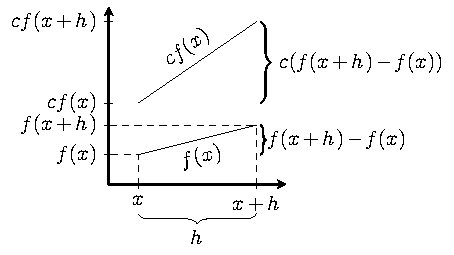
\includegraphics{basicderivativesandintegrals/derivativeconstantmultiple}
        \caption{for derivatives}
        \label{fig:derivativesconstantmultiple}
    \end{subfigure}
    \begin{subfigure}[b]{0.36\textwidth}
        \centering
        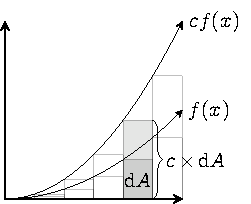
\includegraphics{basicderivativesandintegrals/integralconstantmultiple}
        \caption{for integrals}
        \label{fig:integralsconstantmultiple}
    \end{subfigure}
    \caption{Constant multiple rules}
\end{figure}

It shouldn't be too hard to think of these rules visually because it's just scaling and adding functions together. For any function $f(x)$ and $g(x)$, and constants $a$ and $b$, the following rules follows.
\index{derivatives!constant multiple rule}\index{integrals!constant multiple rule}\paragraph{The constant multiple rules:}
\begin{align}
    \odv*{(af(x))}{x} &= a\odv{f(x)}{x}, &\alc[0.3]{Illustrated in \cref{fig:derivativesconstantmultiple}}\label{eq:derivativesconstantmultiple} \\
    \int af(x)\odif{x} &= a\int f(x)\odif{x}. &\alc[0.3]{Illustrated in \cref{fig:integralsconstantmultiple}}\label{eq:integralsconstantmultiple}
\end{align}

\index{derivatives!sum rule}\index{integrals!sum rule}\paragraph{The sum rules:}
\begin{align}
    \odv*{(f(x) + g(x))}{x} &= \odv*{f(x)}{x} + \odv*{g(x)}{x}, \label{eq:derivativesumrule}\\
    \int f(x) + g(x)\odif{x} &= \int f(x)\odif{x} + \int g(x)\odif{x}. \label{eq:integralssumrule}
\end{align}
The slope of the sum of two functions adds up, and so the area.

Generally, we say that these operations, i.e., the derivative and the antiderivative is \index{linearity of derivatives and antiderivatives}\index{derivatives!linearity |see {linearity of derivatives and antiderivatives}}\index{integrals!linearity |see {linearity of derivatives and antiderivatives}}\textbf{linear} because they have the property
\begin{gather*}
    \mathrm{D}(af(x) + bg(x)) = a\mathrm{D}(f(x)) + b\mathrm{D}(g(x)),
\end{gather*}
where $\mathrm{D}$ is an \index{operator}\textbf{operator}. An operator is like an instruction to do something. Here, $\mathrm{D}$ could represent ``\emph{take the derivative}'', or ``\emph{find the antiderivative}''. You could interpret ``\emph{linear}'' as in derivatives approximate everything as a line (\Cref{remark:derivatives}). The true meaning of this is actually engrained in linear algebra which is beyond the scope of this book. You can consult any linear algebra textbook for it.

\section{Derivatives and antiderivatives of polynomials}

Now that we've discussed the ``trivial rules'', we're ready to tackle the most comprehensive family of functions: the \textbf{polynomials}\index{polynomials}. They're in the form
\begin{equation*}
    f(x) = a_0 + a_1x + a_2x^2 + a_3x^3 + \dots.
\end{equation*}
Because the linearity of both derivatives and antiderivatives, we can break down the polynomial into multiple monomials\index{monomials}. Thus, if we know the derivative and antiderivatives of $x^n$, we basically get the whole family for free.

\subsection{Derivatives of polynomials: the power rule}
\label{sec:derivativespowerrule}

Let's start of with the derivatives. We could use the method of increments every time, but it isn't quite interesting. Therefore, let's focus on the geometrical intuition first by considering the derivative of $x^2$\footnote{Don't worry, if we can find its derivative, we can also find its antiderivative after.}. Geometrically, $x^2$ resembles a square. The derivative question then becomes ``Take a square side length $x$ then, increase its side length by $\odif{x}$. How much area has changed in proportion to $\odif{x}$.''

\begin{figure}[b]
    \centering
    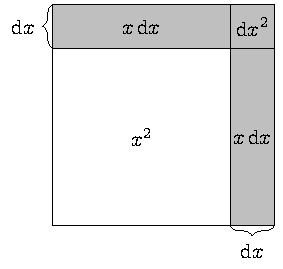
\includegraphics{basicderivativesandintegrals/xsquaredpowerrule}
    \caption{The geometrical interpretation of the derivative of $x^2$}
    \label{fig:xsquaredpowerrule}
\end{figure}
Illustrated in \cref{fig:xsquaredpowerrule}, we can say that
\begin{equation}
    \odv*{(x^2)}{x} = \lim_{\odif{x} \appr 0} \frac{x\odif{x} + x\odif{x} + \odif{x}^2}{\odif{x}}. \label{eq:xsquaredpowerrule}
\end{equation}
Geometrically, the $\odif{x}^2$ square is negligible. When $\odif{x} \appr 0$, that square will just become a single point compared to the big $x\odif{x}$ on the side; therefore, we can safely leave it out. The equation then becomes
\begin{align*}
    \odv*{(x^2)}{x} = \lim_{\odif{x} \appr 0}\frac{2x\odif{x}}{\odif{x}} = 2x:
\end{align*}
the derivative of $x^2$ is $2x$.

Notice, \cref{eq:xsquaredpowerrule} has the same form as if we were to use the method of increments
\begin{equation*}
    \odv*{(x^2)}{x} = \lim_{h\appr 0}\frac{(x + \odif{x})^2 - x^2}{\odif{x}}.
\end{equation*}
This shows that the geometrical method and the symbolical method is equivalent in nature. Now, deriving the derivative of $x^3$ geometrically shouldn't be hard either. Just take a cube side length $x$, then increase its side length by $\odif{x}$ and see how the volume changes in proportion to $\odif{x}$. The final answer should be $3x^2$.

We could go on and derive the derivative of higher powers geometrically using 4-dimensional space. But sadly, we don't have the glory of higher dimensions in our world\footnote{Technically, it's possibly to visualize 4-dimensional space. However, it'd take months to get the hang of it. Not even mentioning the fifth dimension. Therefore, we should leave it off for now.}. To go further without headaches, we turn to the binomial expansion and the mighty definition of derivatives
\begin{equation*}
    \odv{(x^n)}{x} = \lim_{h \appr 0}\frac{(x + h)^n - x^n}{h}.
\end{equation*}
Then, use the binomial expansion (\cref{appendix:binomialexpansion}) on $(x + h)^n$.
\begin{align*}
    &= \lim_{h \appr 0}\frac{\left(\sum_{k = 0}^n{n\choose k}x^{n - k}\cdot h^n\right) - x^n}{h} \\
    &= \lim_{h \appr 0}{{n\choose 0}x^nh^0 + {n\choose 1}x^{n - 1}h^1 + {n\choose 2}x^{n - 2}h^2 +\dots {n\choose n} + x^0h^n - x^n\over h} \\
    &= \lim_{h \appr 0}\frac{x^n + nx^{n - 1}h^1 + {n\choose 2}x^{n - 2}h^2 + \dots + h^n -x^n}{h} \\
    &= \lim_{h \appr 0}nx^{n - 1} + {n\choose 2}x^{n - 2}h + {n\choose 3}x^{n - 3}h^2 + h^{n - 1}
\end{align*}
As $h\appr 0$, the remaining terms would vanish. Thus,
\begin{equation}
    \odv{x}(x^n) = nx^{n - 1}, \label{eq:derivativepowerrule}
\end{equation}
which is what we call the power rule of derivative. I'd like to clarify that binomial theorem does work for all real numbers. The prove is in \cref{appendix:binomialexpansion} if you'd like to take a look for yourself.

Here, I leave some exercises which shouldn't be too hard to do
\begin{enumerate}
    \item $\odv*{(x^2 - 2x + 16)}{x}$ \hfill $2x - 2$
    \item $\odv*{(x^3 + x^2 + x + 1)}{x}$ \hfill $3x^2 + 2x + 1$
    \item $\odv*{(3x^4 + 24x^3 - 2x^2 - 32x + 88)}{x}$ \hfill $12x^3 + 72x^2 - 4x - 32$
\end{enumerate}

\subsection{Antiderivatives of polynomials: the reversed power rule}

Now, we can move on to reversing the power rule. We want to find the antiderivative of $x^n$. By the fundamental theorem of calculus and \cref{eq:derivativepowerrule},
\begin{equation*}
    x^n = \int nx^{n - 1} \odif{x}.
\end{equation*}
Since $n$ is a dummy variable, we can change $n$ to $n + 1$
\begin{equation*}
    \int (n + 1)x^{n}\odif{x} = x^{n + 1},
\end{equation*}
and by the linearity of integrations (\cref{eq:integralsconstantmultiple}), we get the \index{integrals!reversed power rule}\textbf{reversed power rule}:
\begin{equation}
    \int x^{n}\odif{x} = \frac{x^{n + 1}}{n + 1}.
\end{equation}

Notice, this rule does not work for $n = 1$ because we can't divide by zero\dots \emph{or can we???} (Discussed further in \cref{sec:integralofthereciprocal})

\section{Extending the equations of linear motion}

In \cref{sec:fiveequationsoflinearmotion}, we discussed the equation of motion of objects with uniformed acceleration. What if now, the acceleration is changing over time? In a sense, we can use the Newton's second law to deal with that also. If the jerk $j$ is constant, the acceleration must be increasing uniformly
\begin{equation*}
    j = \odv{a}{t}.
\end{equation*}
We can then move $\odif{t}$ around and integrate both sides by using the reversed power rule on it.
\begin{align*}
    \int j\odif{t} &= \int\odif{a} \\
    j\int \odif{t} &= \int\odif{a} \alc[0.35]{Linearity of integrals} \\
    jt + a_0 &= a \alc[0.35]{Integrating an infinitesimal \& Integral constant}
\end{align*}
Then, because $a$ is the derivative of $v$. Note that both $a$, and $v$ is a function of time.
\begin{align*}
    \odv{v}{t} &= jt + a_0 \\
    \int \odif{v} &= \int jt + a_0 \odif{t} \\
    v &= j\int t\odif{t} + \int a_0\odif{t} \alc{Linearity of integrals} \\
    v &= \frac{1}{2}jt^2 + a_0t + v_0. \alc{Reversed power rule \& Integral constant} \\
\end{align*}
Because $v$ is the derivative of $r$,
\begin{align*}
    \odv{r}{t} &= \frac{1}{2}jt^2 + a_0t + v_0 \\
    \int \odif{r} &= \int\frac{1}{2}jt^2 + a_0t + v_0 \odif{t} \\
    r &= \frac{1}{2}j\int t^2\odif{t} + a_0\int t\odif{t} + v_0\int\odif{t} \\
    r &= \frac{1}{6}jt^3 + \frac{1}{2}a_0t^2 + v_0t + r_0.
\end{align*}
And there you have it! Technically we can extend this to whatever we want. The jerk also doesn't have to be uniformed, it could be a function of time itself. But, that's probably enough. If you'd like to try, extend the equation of motion to uniformed snap $s$. The final equation should be
\begin{equation*}
    r = \frac{1}{24}st^4 + \frac{1}{6}jt^3 + \frac{1}{2}a_0t^2 + v_0t + r_0.
\end{equation*}

\section{Exponentials, growth pill}

Let's say there's a magical drop of water that doubles its volume $V$ every hour. That means, for every time $t$,
\begin{equation}
    V(t + 1) = 2V(t). \label{eq:exponentialsrecurrencerelations}
\end{equation}

\begin{wraptable}[12]{r}{0.445\textwidth}
    \centering
    \begin{tabular}{C | C | C}
        t & V(t) & V(t) - V(t - 1) \\
        \hline
        0 & 1 & \\
        1 & 2 & 2 - 1 = 1 \\
        2 & 4 & 4 - 2 = 2 \\
        3 & 8 & 8 - 4 = 4 \\
        4 & 16 & 16 - 8 = 8 \\
        5 & 32 & 32 - 16 = 16 \\
        6 & 64 & 64 - 32 = 32 \\
        7 & 128 & 128 - 64 = 64 \\
        8 & 256 & 256 - 128 = 128 \\
        9 & 512 & 512 - 256 = 256 \\
        10 & 1024 & 1024 - 512 = 12
    \end{tabular}
    \caption{Tables of $2^x$ plotted at interval $1$ from $0$ to $10$}
    \label{tab:exponentialbase2}
\end{wraptable}
We can find the function $V(t)$ that satisfies the function above. Because we're dealing with integers time here, we can consider the function from $V(0)$ to $V(t)$. If we set $V(0) = 1$, that is the drop starts at one unit of volume,
\begin{align*}
    V(1) &= 2V(0) = 2, \\
    V(2) &= 2V(1) = 2(2) = 2^2, \\
    V(3) &= 2V(2) = 2(2^2) = 2^3, \\
    V(4) &= 2V(3) = 2(2^3) = 2^4, \\
    &\vdots
\end{align*}
It's clear that the pattern is $V(t) = 2^t$, which is an exponential function. Because we're in calculus, a natural question to ask is ``\emph{what is its rate of change?}''. So you might start plotting it over time (\cref{fig:exponentialgraph}). However, these exponential grows so quickly that by $V(7)$, we're already in the hundreds. It'd probably be better to list the values of each point on a table.
\begin{figure}[t]
    \centering
    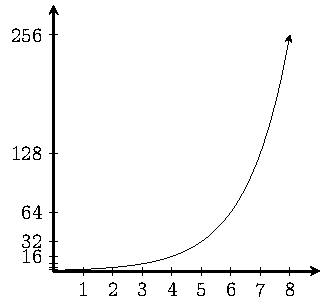
\includegraphics{basicderivativesandintegrals/exponentials}
    \caption{Exponential function $2^x$ plotted from $0$ to $8$}
    \label{fig:exponentialgraph}
\end{figure}
On the right most column of \cref{tab:exponentialbase2}, there's something suspicious going on. Specifically, the difference between $V(t)$ and $V(t - 1)$ is exactly $V(t - 1)$: the function changes as much as its past-self. Does that mean that the derivative of $2^x$ equals $2^x$?

Well, sadly not, but close. See, \cref{tab:exponentialbase2} only shows a \emph{discrete} step. You can write it out as
\begin{equation}
    \frac{2^{x + 1} - 2^x}{1} = 2^x\left(\frac{2 - 1}{1}\right) = 2^x,
\end{equation}
that is why we saw that $V(t) - V(t - 1) = V(t - 1)$. However, if we'd want to calculate the derivative of $2^x$, you'd have to use the method of increments:
\begin{align*}
    \odv*{(2^x)}{x} &= \lim_{h \appr 0}\frac{2^{x + h} - 2^x}{\odif{x}} \\
    &= 2^x\lim_{h \appr 0}\left(\frac{2^h - 1}{h}\right).
\end{align*}
Now you could try plugging in a really small value of $h$, say $0.000001$. The term $\frac{2^h - 1}{h}$ will approach $0.69314\dots$. If you try other bases of exponents, say $3$, you might see a pattern emerging.
\begin{equation}
    \odv*{(3^x)}{x} = 3^x\lim_{h \appr 0}\frac{3^h - 1}{h}.
\end{equation}
\emph{The rate of change of an exponential function is always itself times a proportionality constant}. For $3^x$, it's about $1.09851\dots$. If we could find a number $n$ where $\frac{n^h - 1}{h} = 0$, we'd have a very pretty function which it is its own derivative. So let's find that!
 
\subsection{A function that is its own derivative}
\label{sec:afunctionthatisitsownderivative}

Let's set a goal: find the function that is its own derivative. I shall introduce a substantial concept in calculus: the expansion of functions. Every function has a polynomial expansion\footnote{Although the convergence of the series derived is quite questionable; thankfully, the power series of $n^x$ converges everywhere.} called the \index{power series!introduction}\textbf{power series}. For every $f(x)$,
\begin{equation}
    f(x) = a_0 + a_1x^1 + a_2x^2 + a_3x^3 +\dots. \label{eq:naivetaylorseries}
\end{equation}
E.g., $\sin(x)$ can be written as
\begin{equation}
    \sin(x) = x - \frac{1}{3!}x^3 + \frac{1}{5!}x^5 - \frac{1}{7!}x^7 + \dots. \label{eq:taylorseriessine}
\end{equation}
we will derive this expression later in \cref{sec:taylorseriesforsineandcosine}. For now, we can just use \cref{eq:naivetaylorseries} to find the expression for the function that is its own derivative.

We've seen that the exponential is a possible candidate for a function that is its own derivative. Now, assume that for some real number $n$,
\begin{equation}
    \odv*{(n^x)}{x} = n^x.
\end{equation}
Then, we use the polynomial expansion and the power rule,
\begin{align*}
    \odv*{(a_0 + a_1x^1 + a_2x^2 + a_3x^3 + \dots)}{x} &= a_1 + 2a_2x^1 + 3a_3x^2 + 4a_4x^3 + \dots \\
    &= n^x
\end{align*}
If the function is its own derivative, the polynomial expansion of the function and its derivative must be the same.
\begin{gather}
    n^x = a_0 + a_1x^1 + a_2x^2 + a_3x^3 + \dots, \label{eq:naivetaylorseries1}\\
    n^x = a_1 + 2a_2x^1 + 3a_3x^2 + 4a_4x^3 + \dots. \label{eq:naivetaylorseries2}
\end{gather}
Since both are polynomials, we can match the coefficient here:
\begin{equation}
    \begin{array}{c}
    a_0 = a_1 \\ a_1 = 2a_2 \\ a_2 = 3a_3 \\ a_3 = 4a_4 \\ \vdots
    \end{array}\label{eq:naivetaylorserieserelations}
\end{equation}
$a_0$ and $a_1$ is relatively easy to find. As we've seen, $n$ must be between $2$ and $3$. By the properties of exponentials, $x = 0 \implies n^x = 1$. We can then plug $x = 0$ and set $n^x = 1$ into \cref{eq:naivetaylorseries2}:
\begin{align*}
    1 &= a_0 + a_1(0)^1 + a_2(0)^2 + a_3(0)^3 + \dots \\
    a_0 &= 1.
\end{align*}
Since $a_0 = a_1$, $a_1$ must also be $1$. We can then go back to \cref{eq:naivetaylorserieserelations} and get
\begin{equation*}
    n^x = 1 + 1 + \frac{1}{2!}x + \frac{1}{3!}x^3 + \frac{1}{4!}x^4 + \dots
\end{equation*}
The pattern here is clearly $a_n = n!$. If we want to find $n$, we just let $x = 1$.
\begin{equation*}
    n = 1 + 1 + \frac{1}{2!} + \frac{1}{3!} + \frac{1}{4!} + \dots,
\end{equation*}
and there we have an expression for $n$ which is an irrational number. If you work this out, it's around $2.71828\dots$. Because $(2.71828\dots)^x$ is its own derivative, it's very useful in mathematics and appears everywhere, even at the seams of mathematics that doesn't even seems related to growths: the patterns of prime number, this constant $2.71828\dotso$ has a name and symbol: the Euler's number\footnote{Not to be confused with the ``Euler's constant'' which is another constant written $\gamma$, and is around $0.57721\dots$}, written as $\e$ where
\begin{equation}
    \e = \sum_{i = 0}^{\infty}\frac{1}{i!}
\end{equation}

\subsection{\protect Another interpretation of $\e$: infinite bank interests}

There are two types of bank interests: simple and compound. Simple interests is the thing that you don't really want: the interest is always the same and doesn't grow with your account. You can calculate it by using
\begin{equation}
    n(t) = n_0 + tr
\end{equation}
where $n(t)$ is the total money at time $t$, $n_0$ the initial money in your bank account, and $r$, the interest rate.

Compound interest in the other hand calculates your interest based on how much money you have at that moment:
\begin{equation}
    n(t + 1) = n(t)r + n(t).
\end{equation}
We can find the expression for $n(t)$ in a similar fashion to what we've done in \cref{eq:exponentialsrecurrencerelations}. You'll get
\begin{equation}
    n(t) = (1 + r)^tn_0 \label{eq:compoundinterestformula}
\end{equation}
which is an exponential function.

Let's say you deposit $100\$$ into a bank and the bank is offering you two options on \index{compound interest}\textbf{compound interests} rate. \begin{enumerate*}[label = \arabic*)]\item Take $100\%$ interest in $1$ year, \item Take $\flatfrac{100}{2}\%$ twice a year, or \item Take $\flatfrac{100}{356}\%$ daily.\end{enumerate*} If you take option one, you'd end up with $200\$$. Option two takes you to $225\$$, and option three takes you to around $271.447\dots\$$. You might see a theme here. If you get $\flatfrac{100}{n}\%$ interest, $n$ times a year, the result keeps getting higher. Is there an upper limit to this?

If we write it in terms of limits as $n \appr \infty$ and use \cref{eq:compoundinterestformula}, the compound interests formula,
\begin{equation*}
    x = \lim_{n \appr \infty}\left(1 + \frac{1}{n}\right)^nn_0.
\end{equation*}
Where $x$ is the total money after a year. We're interested in the upper limit, so we'll just let $n_0$ for now. The expression will become
\begin{equation}
    x = \lim_{n \appr \infty}\left(1 + \frac{1}{n}\right)^n \label{eq:infinitecompoundinterest}
\end{equation}
Technically, we could go in and substitute a very high $n$, such as $1000000$. But I believe you could already see that it would be a nightmare to calculate: exponentiation is not at all an easy task. However, notice that from option three earlier, the total money is $271.447\dots\$$ which is suspiciously similar to $\e$ at $2.71828\dots$. If \cref{eq:infinitecompoundinterest} equals \cref{eq:naivetaylorserieserelations}, we'd find the upper limit for this problem and solve the mystery.

We can use the binomial theorem on \cref{eq:infinitecompoundinterest} and get
\begin{align*}
    &\lim_{n \appr \infty}\sum_{k = 0}^{n}{n \choose k}1^{n - k}\frac{1}{n^k} \\
    &= \lim_{n \appr \infty}{n \choose 0}\frac{1}{n^0} + {n \choose 1}\frac{1}{n^1} + {n \choose 2}\frac{1}{n^2} + {n \choose 3}\frac{1}{n^3} + \dots.
\end{align*}
Then, we use the definition of $n$ choose $k$,
\begin{align*}
    &= 1 + \lim_{n \appr \infty}\frac{n!}{1!(n - 1)!}\frac{1}{n^1} + \frac{n!}{2!(n - 2)!}\frac{1}{n^2} + \frac{n!}{3!(n - 3)!}\frac{1}{n^3} + \dots.
\end{align*}
Now, we can cancel the $n!$ on the numerator to the denominator and isolate the factorials.
\begin{align*}
    &= 1 + \lim_{n \appr \infty}\frac{n(n - 1)!}{(n - 1)!}\frac{1}{1!n^1} + \frac{n(n - 1)(n - 2)!}{(n - 2)!}\frac{1}{2!n^2} + \dots \\
    &= 1 + \frac{1}{1!} + \lim_{n \appr \infty} \frac{n(n - 1)}{2!n^2} + \frac{n(n - 1)(n - 2)}{3!n^3} + \frac{n(n - 1)(n - 2)(n - 3)}{4!n^4} + \dots
\end{align*}
Notice, as $n \appr \infty$, the ratio between $n + R$ and $n$ where $R$ is any real numbers would be literally negligible. For every terms in our series, both the numerator and the denominator has the same polynomic degrees. Therefore, all the $n$'s in the series cancel out and we get
\begin{equation}
    x = 1 + \frac{1}{1!} + \frac{1}{2!} + \frac{1}{3!} + \dots
\end{equation}
which is literally \cref{eq:naivetaylorserieserelations}. That means, the upper limit that the bank can give you is $\e$. Geometrically, it should make sense. Because we're gradually turning a discrete interest into a continuous one, $\e$ should appear in the limit of the continuous bank interests.

\subsection{The antiderivative of exponential functions}

It should be trivial that if $\e^x$ is the derivative of itself, so is its antiderivative
\begin{equation}
    \int \e^x \odif{x} = \e^x + C.
\end{equation}
For other bases, we could use \cref{theorem:fundamentalthmofcalc1}, the fundamental theorem of calculus, to find its antiderivative. That is, if
\begin{equation*}
    \odv{(n^x)}{x} = n^x\lim_{h \appr 0}\frac{n^h - 1}{h},
\end{equation*}
then
\begin{align*}
    \odv*{(n^x)}{x} &= n^x\lim_{h \appr 0}\frac{n^h - 1}{h} \\
    n^x &= \lim_{h \appr 0}\frac{n^h - 1}{h}\int n^x\odif{x} \\
    \int n^x\odif{x} &= n^x\lim_{h \appr 0}\left(\frac{n^h - 1}{h}\right)^{-1}.
\end{align*}
The term in the limit sign still appears here. If we want to uncover how this term comes to be, we must discuss the logarithms.

\section{Logarithms}

Monomials has their inverse functions: the roots, exponentials also has an inverse functions: the logarithms. Here's a simple example to illustrate what I mean.
\begin{equation*}
    \sqrt[a]{x^a} = x, \textrm{ but with logarithms, } \log_{a}(a^x) = x.
\end{equation*}
\index{logarithms}\textbf{Logarithms} are inverses functions of exponentials: it cancels exponentials. With it comes the following properties:
\begin{gather}
    \log_a(x) + \log_a(y) = \log_a(xy) \\
    \log_a(x) - \log_a(y) = \log_a\left(\frac{x}{y}\right) \\
    \log_a(x) = \frac{\log_b(x)}{\log_b(a)}
\end{gather}
Since $\e^x$ is shown to be a very important function in modelling continuous growth, and is its own derivative, we give its inverse function its own name: the \index{logarithms!natural logarithms}\textbf{natural logarithm}, written as $\ln(x)$.

So what's the growth of $\ln(x)$? At first sight, since the exponential grows so fast, the inverse of exponentials must grow very slowly. It might just be the reciprocal of $x$: $\flatfrac{1}{x}$. However, we have to derive it somehow. You could try the method of increments and get
\begin{equation}
    \odv{\ln(x)}{x} = \lim_{h \appr 0}\frac{\ln(x + h) - \ln(x)}{h}.
\end{equation}
As seen, there are no properties of logarithm that can manipulate this. However, I shall introduce quite a sneaky concept here called \index{implicit differentiation}\textbf{implicit differentiation}.

Notice that we've only concerned the function that's clearly written in the form $f(x) = y$ and its rate of change. We call these neat functions \index{functions!explicit}\textbf{explicit functions}. However, not all functions are written in this form. E.g., $\sqrt{x^2 + y^2} = 2$. These functions are called \index{inplicit functions}\textbf{implicit functions}, and we can actually differentiate it.

If I let $\ln(x) = y$, I can raise $\e$ to the power of both sides and get
\begin{equation}
    \e^{\ln(x)} = \e^y.
\end{equation}
Because logarithms are inverses of exponentials,
\begin{equation}
    x = \e^y.
\end{equation}
If you remember from \cref{sec:rulesofequality}, if two sides of the equation are equal, their derivatives with respect to the same variable must also be equal. We can take its derivative with respect to $y$ instead of $x$:
\begin{align*}
    \odv{x}{y} &= \odv{\e^y}{y} \\
    \odv{x}{y} &= \e^y.
\end{align*}
But we're looking for the derivative of $y$ (which is just $\ln(x)$) w.r.t. $x$, not the derivative of $x$ w.r.t. $y$. Here's where Leibniz's notation comes into clutch: we can swap the numerator with the denominator for both sides then substitute in the $y$:
\begin{align*}
    \odv{\ln(x)}{x} &= \frac{1}{\e^{\ln(x)}} \\
    \therefore~\odv{\ln(x)}{x} &= \frac{1}{x},
\end{align*}
and there: the derivative of the natural logarithm is the reciprocal.

With the power of natural logarithms, we can actually go back at the derivative of $n^x$ and finally uncover the mystery behind the proportionality term that's lingering around. Start with the manipulation of $n^x$.
\begin{equation}
    n^x = \left(\e^{\ln(n)}\right)^x = \e^{x\ln(x)}.
\end{equation}
With the chain rule, discussed in \cref{sec:thechainrule}, we can let $u = x\ln(n)$ and add an intermediate step:
\begin{align*}
    \odv{x}(n^x) &= \odv{\e^{x\ln(n)}}{x} \\
    &= \odv{\e^u}{x} \times \odv{u}{u} \\
    &= \odv{\e^u}{u} \times \odv{u}{x} \\
    &= \e^{x\ln(n)} \times \odv{x\ln(n)}{x} \\
    &= n^x\ln(n).
\end{align*}
And here it is. The mystery proportionality constant is just a consequence of the natural logarithm. Thus, one way to define the natural log would be
\begin{equation}
    \ln(n) = \lim_{h \appr 0}\frac{n^h - 1}{h}.
\end{equation}
The antiderivative of other bases exponents are then given by
\begin{equation}
    \int n^x = \frac{1}{\ln(n)}n^x + C.
\end{equation}

\subsection{The product rule and the quotient rule}
\index{derivatives!product rule}

Sometimes, we have to multiply the two functions together before taking the derivatives. There are two ways to do this. To keep the spirit of visualization, I shall first introduce the geometrical way, then the analytical way.

\begin{figure}[h]
    \centering
    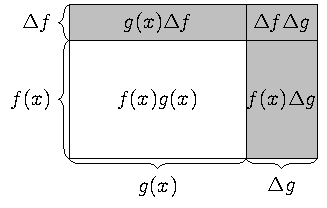
\includegraphics{basicderivativesandintegrals/derivativesproductrule}
    \caption{The geometrical interpretation of the product rule.}
    \label{fig:derivativesproductrule}
\end{figure}
The derivative of $f(x)g(x)$ w.r.t. $x$ can be thought of a rectangle with side length that's governed by $f(x)$ and $g(x)$. As shown in \cref{fig:derivativesproductrule}, the area increase on side $f(x)$ is $g(x)\Dd{f}$ and on $g(x)$, $f(x)\Dd{g}$. The $\Dd{f}\Dd{g}$ part is basically negligible. Therefore,
\begin{align*}
    \odv*{(f(x)g(x))}{x} &= \lim_{h \appr 0}\frac{g(x)\Dd{f} + f(x)\Dd{g}}{h} \\
    &= \lim_{h \appr 0}\frac{f(x)(g(x + h) - g(x)) + g(x)(f(x + h) - f(x))}{h} \\
    &= f(x)\lim_{h \appr 0}\frac{g(x + h) - g(x)}{h} + g(x)\lim_{h \appr 0}\frac{f(x + h) - f(x)}{h} \\
    &= f(x)\odv{g(x)}{x} + g(x)\odv{f(x)}{x}.
\end{align*}
Which is what we call the product rule. Notice the alternation between $f$ and $g$ in the two terms. The derivative of $f(x)$ is multiplied by $g(x)$, and the derivative of $g(x)$ is multiplied by $f(x)$. This is a direct consequence of the diagram: the change in $f(x)$ is multiplied by $g(x)$ to give the area and also the other way around. You could check this with the method of increments, and it would still be true. I encourage you to do it.

\index{derivatives!quotient rule}To take derivatives of quotients of functions, just plug in $\flatfrac{1}{g(x)}$ instead of $g(x)$. The final form should be
\begin{equation}
    \odv*{\ab(\frac{f(x)}{g(x)})}{x} = \frac{\displaystyle f(x)\odv{g(x)}{x} - g(x)\odv{f(x)}{x}}{f(x)^2}.
\end{equation}

But how's about the product of three functions, e.g., $a(x)b(x)c(x)$? Or even more functions multiplied together? Well we ran into the same problem as what we were doing earlier in \cref{sec:derivativespowerrule}, deriving the power rule: we don't have enough dimensions. So sadly, we have to turn ourselves to analytical method.

Let's think of this through. We still don't know how to take derivatives of products of multiple functions. However, we know the derivatives of \emph{sums} of multiple functions by the linearity property. So if we can turn products into sum, this problem would be our candy. Gladly, there's a function that can do exactly that: the logarithms. To make our life easier, we shall use the natural logarithm. Because I want to save space, let's write $a(x)b(x)c(x)$ as just $abc$. Do know that these functions are all dependent on $x$. Start off with a manipulation of products.
\begin{align*}
    \odv{(abc\dots)}{x} &= \odv*{(e^{\ln(abc\dots)})}{x} \\
    &= \odv*{(\e^{\ln(a) + \ln(b) + \ln(c) + \dots})}{x}.
\end{align*}
Now, let $\ln(a) + \ln(b) + \ln(c) + \dots = u$ and use the chain rule,
\begin{align*}
    &= \odv*{(\e^u)}{x} \cdot \odv{u}{u} \\
    &= \odv*{(\e^u)}{x} \cdot \odv*{\ab(\ln(a) + \ln(b) + \ln(c) + \dots)}{x} \\
    &= \e^u \left(\odv{\ln(a)}{x} + \odv{\ln(b)}{x} + \odv{\ln(c)}{x} + \dots\right).
\end{align*}
Then use the chain rule again on the terms in the parenthesis
\begin{align*}
    &= \e^u \left(\odv{\ln(a)}{x}\odv{a}{a} + \odv{\ln(b)}{x}\odv{b}{b} + \odv{\ln(c)}{x}\odv{c}{c} + \dots\right) \\
    &= (abc\dots)\left(\odv{\ln(a)}{a}\odv{a}{x} + \odv{\ln(b)}{b}\odv{b}{x} + \odv{\ln(c)}{c}\odv{c}{x} + \dots\right) \\
    &= (abc\dots)\left(\frac{1}{a}\odv{a}{x} + \frac{1}{b}\odv{b}{x} + \frac{1}{c}\odv{c}{x} + \dots\right).
\end{align*}
And there we have it: the generalized product rule.

\subsection{Alternate derivations for the power rule}

The power rule can also be derived using the same techique we just used. However, we use a different property of logarithm: $\ln(x^n) = n\ln(x)$.
\begin{equation*}
    \odv{x^n}{x} = \odv{\e^{n\ln(x)}}{x}.
\end{equation*}
Let $n\ln(x) = u$ then use the chain rule
\begin{align*}
    &= \odv{\e^u}{x} \cdot \odv{u}{u} \\
    &= \odv{\e^u}{u} \cdot \odv{u}{x} \\
    &= \e^u \cdot \odv*{\ab(n\ln(x))}{x} \\
    &= x^n \cdot n\frac{1}{x} = nx^{n - 1}.
\end{align*}

\section{Implicit differentiation}

We've discussed that we can differentiate implicit functions. Normally, it wouldn't be quite useful, but this \index{derivatives!implicit differentiation}\textbf{implicit differentiation} shows up when two rates of change are related to each other: the \textbf{related rates} problem.

Take the example of a sliding ladder, sketched in \cref{fig:slidingladder}. The ladder is $5\unit{\meter}$ long. If any one moment, what is the rate of sliding along the $x$-axis w.r.t. the $y$-axis?

\begin{figure}
    \centering
    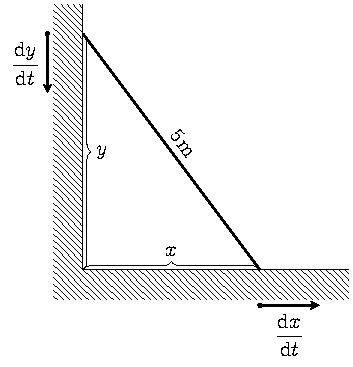
\includegraphics{basicderivativesandintegrals/slidingladder}
    \caption{A ladder length $5\unit{\meter}$ sliding down a corner.}
    \label{fig:slidingladder}
\end{figure}

The problem is asking us to find $\odv{x}{y}$. Here, the rates of sliding along the $y$-axis $\odv{y}{t}$ and along the $x$-axis $\odv{x}{t}$ is clearly related because the ladder length still stays the same over time. If $y$ decreases, $x$ must increase. Both variables are related by the Pythagorean theorem
\begin{equation}
    x^2 + y^2 = 5^2.
\end{equation}
Then, we can differentiate this w.r.t. $t$, and use the chain rule
\begin{align*}
    \odv{x^2}{t} + \odv{y^2}{t} &= \odv{(5^2)}{t} \\
    \odv{x^2}{x}\odv{x}{t} + \odv{y^2}{y}\odv{y}{t} &= 0 \\
    2x\odv{x}{t} + 2y\odv{y}{t} &= 0.
\end{align*}
We can take advantage of the Leibniz's notation and multiply by $\odif{t}$ on both sides giving
\begin{equation*}
    2x\odif{x} + 2y\odif{y} = 0.
\end{equation*}
To find $\odv{x}{y}$, we just have to isolate the variables,
\begin{align*}
    \odv{x}{y} = -\frac{y}{x}.
\end{align*}
And this should actually make sense. Because if $y$ is increasing by a bit, $x$ must decrease by some amount, and that amount is $-\flatfrac{y}{x}$: the higher the $y$, the larger the rates of sliding.

\section{But why is the integral of the reciprocal the natural logarithm?}
\label{sec:integralofthereciprocal}

\index{integrals!integrals of the reciprocal}
\begin{wrapfigure}{r}{0.45\textwidth}
    \centering
    \begin{tabular}{c | c}
        Function & Antiderivative \\
        \hline
        $x^{-3}$ & $-\flatfrac{x^{-2}}{2}$ \\
        $x^{-2}$ & $x^{-1}$ \\
        $x^{-1}$ or $\flatfrac{1}{x}$ & $\ln(x)$ \\
        $x^{0}$ or $1$ & $x$ \\
        $x^1$ & $\flatfrac{x^2}{2}$ \\
    \end{tabular}
    \caption{Tables of reversed power rule from $x^{-3}$ to $x^1$}
\end{wrapfigure}
As we've seen, the antiderivative of $\frac{1}{x}$ is $\ln(x)$ by the fundamental theorem of calculus (\cref{theorem:fundamentalthmofcalc1}). I, however, find it disturbing and unresolved. It's a hole in the reversed power rule. From this dissatisfaction, I spent a night coming up with a way to derive this using just the reversed power rule. Enjoy the transformation!
\begin{align}
    \int \frac{1}{x}\odif{x} &= \int\lim_{h \appr 0}\left(\frac{1}{2}x^{-1 + h} + \frac{1}{2}x^{-1 - h}\right) \nonumber\\
    &= \lim_{h \appr 0}\int\left(\frac{1}{2}x^{-1 + h} + \frac{1}{2}x^{-1 - h}\right) \nonumber\\
    &= \lim_{h \appr 0}\int\left(\frac{1}{2}\frac{x^{-1 + h + 1}}{(-1 + h + 1)} + \frac{1}{2}\frac{x^{-1 - h + 1}}{(-1 - h + 1)}\right) \nonumber\\
    &= \lim_{h \appr 0}\left(\frac{1}{2}\frac{x^h}{h} - \frac{1}{2}\frac{x^{-h}}{-h}\right) = \lim_{h \appr 0}\left(\frac{1}{2}\frac{x^h}{h}\frac{x^h}{h} - \frac{1}{2}\frac{1}{hx^h}\right) \nonumber\\
    &= \lim_{h \appr 0}\left(\frac{x^{2h} - 1}{2hx^h}\right) = \lim_{h \appr 0}\left(\frac{\e^{2h\ln(x)} - 1}{2h\ln(x)}\cdot\frac{\ln(x)}{x^h}\right) \nonumber\\
    &= \lim_{h \appr 0}\left(\frac{e^{2h\ln(x)}}{2h\ln(x)}\right) \cdot \lim_{h \appr 0}\left(\frac{\ln(x)}{x^h}\right) \nonumber\\
    &= \lim_{h \appr 0}\left(\frac{e^{2h\ln(x)}}{2h\ln(x)}\right) \cdot \ln(x). \label{eq:logarithmsprove1}
\end{align}
Then, we evaluate the limit at the front by letting $u = 2h\ln(x)$. When $h \appr 0$, $u \appr 0$ aswell. Then, use the definition of $\e$ from \cref{eq:infinitecompoundinterest}.
\begin{align*}
    \lim_{h \appr 0}\left(\frac{\e^{2h\ln(x)}}{2h\ln(x)}\right) &= \lim_{u \appr 0}\left(\frac{\e^u - 1}{u}\right) \\
    &= \lim_{u \appr 0}\left(\frac{\left(\lim_{n \appr \infty}\left(1 + \frac{1}{n}\right)^n\right)^u}{u}\right).
\end{align*}
Change the limits from $n \appr \infty$ into $n \appr 0$. Notice, $\lim_{n \appr 0}\left(1 + \frac{1}{n}\right)^n = \lim_{n \appr 0}\left(1 + n\right)^{\flatfrac{1}{n}}$. If $n \appr 0$ and $u \appr 0$, that means $n = u$. Substitute $n = u$ into the limit,
\begin{align*}
    &= \lim_{u \appr 0}\left(\frac{\left(\lim_{u \appr 0}(1 + u)^{\flatfrac{1}{u}}\right)^u - 1}{u}\right) \\
    &= \lim_{u \appr 0}\left(\frac{1 + u - 1}{u}\right) = 1.
\end{align*}
Then, substitute this limit back into \cref{eq:logarithmsprove1}, you'll see that
\begin{equation*}
    \int\frac{1}{x}\odif{x} = \lim_{h \appr 0}\left(\frac{\e^{2h\ln(x)}}{2h\ln(x)}\right) \cdot \ln(x) = \ln(x) + C.
\end{equation*}

\section{Formula for Chapter \thechapter}

\everymath{\displaystyle}
\subsection{Formula for derivatives of functions}

\begin{enumerate}
    \item $f(x) = g(x) \implies \odv{f(x)}{x} = \odv{g(x)}{x}$ (Rules of Equality)
    \item For $c \in \mathbb{R}$, $\odv{(c)}{x} = 0$ (Derivative of a constant)
    \item $\odv{x}{y} = \odv{x}{u} \times \odv{u}{y}$ (Chain rule)
    \item $\odv*{\ab(af(x) + bg(x))}{x} = a\odv{f(x)}{x} + b\odv{g(x)}{x}$ (Linearity of differentiation)
    \item $\odv*{(ax^n)}{x} = anx^{n - 1}$ (Power rule)
    \item $\odv*{(n^x)}{x} = n^x\ln(n)$, $\odv{(\e^x)}{x} = \e^x$ (Derivative of exponentials)
    \item $\odv*{(\ln(x))}{x} = \frac{1}{x}$ (Derivative of natural logarithms)
    \item $\odv*{(f_1f_2\dots f_n)}{x} = f_1f_2\dots f_n\ab(\frac{1}{f_1} + \frac{1}{f_2} + \dots + \frac{1}{f_n})$ (Generalized product rule)
\end{enumerate}

\subsection{Formula for antiderivatives of functions}

\begin{enumerate}
    \item $f(x) = g(x) \implies \int f(x)\odif{x} = \int g(x)\odif{x}$ (Rules of Equality)
    \item $\int af(x) + bg(x) \odif{x} = a\int f(x)\odif{x} + b\int g(x)\odif{x}$ (Linearity of integration)
    \item $n \neq -1$, $\int ax^n\odif{x} = a\frac{x^{n + 1}}{n + 1} + C$ (Reversed power rule)
    \item $\int n^x\odif{x} = \frac{1}{\ln(n)}n^x + C$, $\int \e^x\odif{x} = \e^x + C$ (Antiderative of exponentials)
    \item $\int \frac{1}{x}\odif{x} = \ln(x) + C$ (Antiderivative of natural logarithms)
\end{enumerate}

\subsection{Definition for various functions and constants}

\begin{enumerate}
    \item $\e^x = \lim_{k \appr 0}\sum_{i \appr 0}^{k}\frac{1}{i!}$
    \item $\e = \lim_{n \appr \infty}\left(1 + \frac{1}{n}\right)^n$
    \item $\ln(x) = \lim_{n \appr 0}\left(\frac{x^h - 1}{h}\right)$
\end{enumerate}

\everymath{\textstyle}